\documentclass{ufsctex/ufsctex}
\usepackage{graphics}
\usepackage{graphicx}
\usepackage{enumitem}
\usepackage{float}
\usepackage[cache=false]{minted}
\usepackage{pgfplots}
\usepackage{smartdiagram}
\usepackage{tikz}
\usetikzlibrary{shapes,decorations,arrows,patterns}
\tikzstyle{decision} = [diamond, draw, fill=blue!20, text width=4.5em, text badly centered, node distance=3cm, inner sep=0pt]
\tikzstyle{block} = [rectangle, draw, fill=blue!20, text width=5em, text centered, rounded corners, minimum height=4em]
\tikzstyle{line} = [draw, -latex']
\tikzstyle{oval} = [draw, ellipse,fill=red!20, node distance=3cm, minimum height=2em]
\title{Estudo sobre o uso da linguagem GraphQL na composição de dados através de serviços baseados em JSON}
\begin{document}
\instituicao[a]{Universidade Federal de Santa Catarina}
\departamento[o]{Departamento de Informática e Estatística}
\curso[o]{Programa de Graduação em Sistemas de Informação}
\documento[o]{{Trabalho de Conclusão de Curso}}
\titulo{Estudo sobre o uso da linguagem GraphQL na composição de dados através de serviços baseados em JSON}
\autor{Mateus Maso}
\grau{Bacharel em Sistemas de Informação}
\local{Florianópolis, SC}
\data{\today}
\orientador{Prof. Dr. Frank Augusto Siqueira}

\capa
\folhaderosto

% \epigrafe{
  Time has told me not to ask for more,
  someday our ocean will find its shore
} {(Nick Drake)}

\paginaepigrafe

\begin{resumo}
  Para acomodar a rápida transformação na demanda por dados em aplicações distribuídas, recentemente tem-se discutido novas maneiras de disponibilizar dados para o consumo eficiente de clientes diversificados. Contudo, as atuais formas de comunicação cliente-servidor têm causado dependência e acoplamento entre o código de busca de dados e a especificação utilizada para acesso da API. Isso porque, para garantir a integridade da comunicação, clientes e serviços precisam estabelecer um contrato de interface de acesso para que não haja mudanças após a implementação do cliente. Para evitar isso, este projeto realiza um estudo sobre o uso da linguagem GraphQL para propor um modelo de comunicação cliente-servidor que não dependa de contrato de API e permita a composição de serviços na busca de dados JSON. Além disso, é desenvolvido uma ferramenta com base no modelo proposto para validar sua aplicabilidade. \\ \\
  \textbf{Palavras-chaves}: GraphQL. REST. JSON Schema.
\end{resumo}
\begin{resumo}[Abstract]
  \begin{otherlanguage*}{english}
  (Arrumar) In order to embrace the growing transformations of flow in which data is access by clients over APIs Web, services that exposes these data had applied efforts in adapt interfaces to  efficient ways to expose data for a diversified consumption of clients. However, the current client implementation approach of the client-server communication model has created dependency and coupling between the client's data fetching code and the API specification used for access. To solve that, this project studies the usage of GraphQL language and API description formats to offer a new cliente-server communication model that avoid coupling due to client fetching code implementation. By automating queries, the model aims to optimize requests, be tolerant of API changes and help fetch data through service composition. Furthermore, a tool is developed based on the proposed model to validate it's aplicability. \\ \\
    \textbf{Key-words}: GraphQL. REST. JSON Hyper-Schema.
  \end{otherlanguage*}
\end{resumo}

\listoffigures
\cleardoublepage
\listoftables*
\cleardoublepage

\begin{siglas}
  \item[AST] Árvore sintática abstrata
  \item[API] Interface de Programação de Aplicação
\end{siglas}
\cleardoublepage

\tableofcontents*
\cleardoublepage

\sumario
\textual

\chapter{Introdução}

% - O crescimento das “API’s”
% 	- Estatisticas sobre o mercado
% 		- numeros sobre crescimento
% 		- numeros sobre distribuiçao de estilos
% 		- numeros sobre projeções futuras
% 	- Por que ocorreu isso?
% 		- SOA is the way to go
% 		- “dev is shifting more and more to the client.”
% 		- companies want get faster into new platforms.
% 	- Qual problema isso está causando?
% 		- Clientes dependentes de tipos/estilos de serviço
% 	- Por que isso é ruim?
% 		- (Perf) Estilos de API podem estar sendo sub/super utilizadas devido a constante mudança fluxo de dados em que clientes vivem.
% 		- (Inovação) Investir em novos modelos/tipos/estilos requer tempo para analisar o impacto no cliente.
% 		- (Agile) APIs tendem a crescer verticalmente e adicionar features em serviços “monoliticos” podem atrasar o crescimento de uma organização.
% 	- Como resolver isso?
% 		- Impedir que o cliente tenha acesso direto as APIs
% 	- De que forma?
% 		- Criar uma ferramenta intermediária responsável por transformar dependencias de entidades em requisições para os serviços.
% 	- Além disso, o que a ferramenta promove?
% 		- Experimentação, adoçao e composição de APIs
% 		- Desenvolvimento continuo no cliente
% 		- Documentação de API’s em formatos machine-readable
% 		- Despreocupação em entender o fluxo de dados
% 		- Aumentar tempo de resposta diminuindo o tráfego e dados.
% 		- Avisos sobre problemas e melhorias na comunicação.
% 		- Uso de microserviços ao invés de serviços monoliticos

%   Its been slowly creeping up on us, creating exciting new possibilities for our applications; APIs are changing the face of the Web.

%   The web has essentially become a service oriented platform, where information and functionality is a available through an API; the Web succeeded where the enterprise largely failed.

%   This success can be attributed to the fact that the web has been decentralized in its approach and has adopted less stringent technologies to become service oriented. Many early APIs were written using SOAP but now REST is the dominant force (though some are more REST than others).  The publication of REST APIs has been rapidly increasing.

%   Some offer both SOAP and REST APIs, but this practice has been on the decline and REST is now preferred for most new APIs.

%   [How REST replaced SOAP on the Web: What it means to you]
%   [http://www.infoq.com/articles/rest-soap]

\section[Descrição do Problema]{Descrição do Problema}

O mercado de API's web transformou o modo de comunicação entre aplicações distribuídas para busca de informações e execução de operações na web. Não é de hoje que organizações tem se preocupado em disponibilizar API's de suas aplicações em forma de serviços para consumo próprio e/ou de terceiros. Empresas como Facebook e Netflix mostram que construir uma aplicação em forma de serviço e disponibilizar uma interface de acesso é essencial para entrar rápido no mercado de plataformas emergentes, oferecer uma melhor experiência para o usuário através do desenvolvimento de clientes nativos, além de agregar valor em seu modelo de negócio ao disponibilizar dados e operações para o uso de terceiros. (ART, 2016)

Segundo ProgrammableWeb, um dos motivos que contribuiu para o aumento do número de API's de serviços foi após a introdução em 2001 do estilo de arquitetura REST. Contudo, após 15 anos de sua introdução e diversos clientes escritos com base em seu protocolo de comunicação, REST tem-se mostrado uma solução ineficiente para lidar com o acesso de estrutura de dados por um grande número de clientes diversificado. Visto que sua interface de acesso é pré-determinada, após publicado, tornando-se difícil prever a demanda de dados e realizar mudanças no fluxo sem que haja versionamento. (ProgrammableWeb, 2016)

Por outro lado, ferramentas como GraphQL (Facebook) e Falcor (Netflix) surgem com o objetivo de resolver este problema mas encontram uma baixa adoção por não conseguirem minimizar a custosa transição que clientes desenvolvidos em REST precisam passar para fugir desta arquitetura.

\section[Objetivos]{Objetivos}

O objetivo deste trabalho é o desenvolvimento de uma ferramenta que ajude na prevenção do acoplamento entre clientes e API's causado pela escrita de código voltado ao acesso direto de estruturas de dados JSON. Além disso, através da análise de metadados, poder oferecer uma maneira genérica (usando GraphQL) para busca dados independente do estilo de arquitetura e fluxo de dados implementado pela API. \\

\textbf{Objetivos específicos} \\

\begin{itemize}
\item Prevenir a mudança de código em clientes devido à alterações na implementação do fluxo de dados por uma API.
\item Facilitar a transição de código em clientes ao atualizar para uma nova versão implementado por uma API.
\item Facilitar a transição de código em clientes ao atualizar para um novo estilo de arquitetura implementado por uma API.
\item Oferecer uma maneira de composição de estruturas de dados entre mais de um serviço e interface de aplicação.
\item Promover a documentação e descrição de metadados em API's. \\
\end{itemize}

\textbf{Limites da pesquisa} \\

\begin{itemize}
\item Foco exclusivo no formato JSON para representação de dados.
\item Foco exclusivo na linguagem GraphQL para consulta de dados.
\item Foco exclusivo no estilo de arquitetura REST para realizar testes.
\item Foco exclusivo na ferramenta JSON Hyper-Schema para descrição de API's REST.
\item Foco exclusivo em validar a ferramenta através de testes para prevenir a mudança de código em clientes devido à alterações na implementação do fluxo de dados por uma API.
\end{itemize}
\section[Metodologia]{Metodologia}

Problema surgiu ao tentar integrar GraphQL em um cliente que fazia requisições à uma API RESTful. Cliente estava completamente acoplado ao fluxo de dados, sendo que a estrutura de dados era a mesma. Como resolver isso?

Prox etapa foi a idealização do projeto. Estudar se era possível resolver esse problema e de que forma. Como criar uma ferramenta que fizesse essa intermediação. GraphQL se tornou uma dependência essencial para o sucesso da ferramenta.

Seguido, foi pensado na criação de uma interface para a ferramenta que fosse fácil de usar, rodasse em serviços GraphQL existentes e pudesse funcionar em API's REST que possuem descrição em linguagens/formatos populares e completos.

Após isso foi feito a implementação para Proof of Concept. Depois que validado, comecei a escrita da monografia e preparação de um ambiente de validação que pudesse enfatizar problemas reais na mudança fluxo de dados entre cliente e servidor. Coletar os dados, analisar e apresentar para comprovação da tese.
\section[Organização do Texto]{Organização do Texto}

O texto está organizado em 6 capítulos. O primeiro aborda os conceitos de fundamentos utilizados para entender o processo de desenvolvimento da ferramenta. Em seguida, em um capítulo a parte, será descrito a tecnologia GraphQL. Após os fundamentos, será descrito todo o processo de desenvolvimento da ferramenta, como a planejamento do projeto, implementação e validação. Após definir o ambiente de validação, será executado os testes de validação, coletado os dados e analisados no capítulo de resultados. Por fim, no último capítulo, será feito um comentário geral sobre o projeto, além de propor melhorias a serem feitas na ferramenta para trabalhos futuros.


\chapter{Fundamentos}

Neste capítulo são estabelecidos os principais conceitos utilizados ao longo do projeto. Será feito uma breve abordagem sobre os fundamentos de serialização de dados; seguido pelo formato de representação JSON; o estilo de arquitetura baseado em recursos REST, além da ferramenta GraphQL para consulta de dados sob demanda.

\section[Serialização de Dados]{Serialização de Dados}

Na ciência da computação, serialização de dados é um processo de tradução usado para converter estruturas de dados\footnote{
  Uma estrutura de dados é uma forma abstrata de representar e organizar dados. Seu objetivo é ajudar a reduzir complexidade, podendo armazenar dados de diferentes tipos, como números, strings ou até mesmo outras estruturas de dados.
} em formatos que possam ser armazenados, transmitidos e reconstruídos por um mesmo ou outro ambiente computacional. \cite{Cline2016}

Dados serializados normalmente vivem mais tempo que suas aplicações de origem e, ao ser armazenado em disco ou transmitido pela rede, são representados de modo diferente que sua estrutura em memória. Para se ler dados serializados em memória é preciso realizar o processo inverso, também chamado de deserialização, onde estes passam a ser representados por estruturas da linguagem de execução. \cite{Guller2016}

\begin{figure}[H]
  \centering
  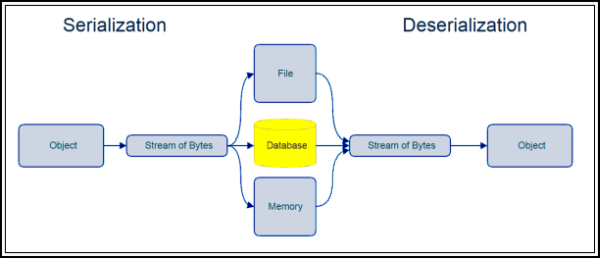
\includegraphics[width=\textwidth,height=\textheight,keepaspectratio]{figuras/data-serialization-deserialization.png}
  \caption{Processo de serialização e deserialização}
\end{figure}

Este processo, embora demande tempo, permitiu que aplicações fizessem o consumo de informações de forma distribuída, contribuindo com o aumento do volume de dados que circulam pela internet. Além disso, fez-se necessário a seleção adequada de formatos de serialização cuja estrutura não prejudique o desempenho de aplicações na busca por dados. \cite{SumarayMakki2012}

Segundo a Cisco Systems\footnote{
  Empresa de sistemas de rede.
}, no ano de 2015, houve um aumento de 21\% no volume de tráfego de dados registrados apenas por seus aparelhos. Sendo a categoria Web, Email e Data responsável por representar aproximadamente 7,558 petabytes de dados transmitidos por seus clientes durante um mês. \cite{Cisco2016}

Para suprir esta alta demanda, diversos formatos de serialização foram introduzidos para melhor atender os problemas de desempenho experienciados por serviços que disponibilizam dados serializados. Dentre eles, tempo de serialização e deserialização, tamanho de transferência, flexibilidade de uso, facilidade de leitura, automação, suporte para linguagem, entre outros. Contudo, cada formato possui seus prós e contras. \cite{Guller2016}

\begin{table}[ht!]
  \centering
  \resizebox{\columnwidth}{!}{
    \begin{tabular}{|c|c|c|c|c|}
      \hline
      Formato & Especificação & Codificação & Human-Readable & Esquema/IDL \\
      \hline
      XML & Padronizada & Textual & Sim & Sim \\
      JSON & Padronizada & Textual & Sim & Parcial \\
      YAML & Padronizada & Textual & Sim & Parcial \\
      Avro & Padronizada & Binário & Não & Sim \\
      Protocol Buffers & Padronizada & Binário & Parcial & Sim \\
      Thrift & Não Padronizada & Binário & Parcial & Sim \\
      \hline
    \end{tabular}
  }
  \caption{Comparação de formatos de serialização}
\end{table}

Para melhor entender o que define cada formato, será feito uma abordagem sobre as categorias de classificação usadas para estudar o comportamento dos formatos existentes hoje.

\input{capitulos/fundamentos/serializacao-de-dados/especificacao/index}
\input{capitulos/fundamentos/serializacao-de-dados/codificacao/index}
\input{capitulos/fundamentos/serializacao-de-dados/human-readable/index}
\input{capitulos/fundamentos/serializacao-de-dados/esquema-idl/index}

\section{JSON}

JSON ou Javascript Object Notation é um formato de serialização de dados human-readable baseado em texto com especificação padronizada e parcialmente descritivo. Foi desenvolvido por Douglas Crockford com o objetivo de representar dados em uma maneira simples, leve e flexível através da redução na sobrecarga de marcações comparado ao formato XML.

Por ter se adaptado bem no ambiente de aplicações distribuídas, este formato acabou sendo amplamente utilizado em serviços como principal forma de representação de dados serializados. \cite{Duvander2013}

Na sua essência, o JSON foi construído com base em quatro tipos primitivos de dados e outros dois para composição. Cada tipo possui seu respectivo correspondente na maioria das linguagens de programação, embora possam ser identificados por nomes diferentes. \cite{Droettboom2015}

\begin{table}[H]
  \centering
  \begin{tabular}{|c|c|c|c|c|}
    \hline
    Tipo & Exemplo de Valor \\
    \hline
    object & \mintinline[fontsize=\small]{c}{ {"chave1": "valor1", "chave2": "valor2"} } \\
    \hline
    array & \mintinline[fontsize=\small]{c}{ ["primeiro", "segundo", "terceiro"] } \\
    \hline
    number & \mintinline[fontsize=\small]{c}{ 1, -1, 2.9999 } \\
    \hline
    string & \mintinline[fontsize=\small]{c}{ "Isso é uma string" } \\
    \hline
    boolean & \mintinline[fontsize=\small]{c}{ true, false } \\
    \hline
    null & \mintinline[fontsize=\small]{c}{ null } \\
    \hline
  \end{tabular}
  \caption{Tipos de valores em JSON}
\end{table}

Através da composição de listas, objetos e tipos primitivos, consegue-se representar complexas estruturas de dados. Não existe, no entanto, um único padrão de representação. Dada uma estrutura, é possível representá-la de inúmeras maneiras. A seguir estão duas formas diferentes de representação em JSON de uma entidade “pessoa”:
 \cite{Droettboom2015}

\begin{figure}[H]
  \centering
  \begin{minted}[frame=single,framesep=10pt,fontsize=\small]{javascript}
    {
      "nome": "Mateus Maso",
      "aniversario": "25 de março de 1992",
      "cidade": "Florianópolis, SC, Brasil"
    }
  \end{minted}
  \caption{Primeiro exemplo de representação JSON}
\end{figure}

\begin{figure}[H]
  \centering
  \begin{minted}[frame=single,framesep=10pt,fontsize=\small]{javascript}
    {
      "nome": "Mateus",
      "sobrenome": "Maso",
      "nascimento": "25-03-1992",
      "cidade": {
        "nome": "Florianópolis",
        "estado": "SC",
        "pais": "Brasil"
      }
    }
  \end{minted}
  \caption{Segundo exemplo de representação JSON}
\end{figure}

Ambas representações são válidas, apesar da figura 4 estar representando os dados em uma estrutura um pouco mais formal. No entanto, por ser um formato não descritivo, a responsabilidade de entender o que está sendo representado vai depender da análise crítica ou conhecimento prévio dos desenvolvedores. Já uma máquina, sem conhecer o contexto, não saberia como interpretar os dados de forma correta. \cite{Droettboom2015}

Para resolver isso, será abordado em seguida um dos formatos existentes hoje em dia para a descrição de estruturas JSON.

\section{REST}

REST ou Representational State Transfer é um estilo arquitetural usado para a comunicação de sistemas distribuídos através do protocolo HTTP. Foi introduzido por Roy Fielding em 2000 com o objetivo de oferecer às aplicações web um modelo de interface de acesso baseada em recursos. Além disso, descreve 6 tipos de restrições que serviços deveriam aplicar para ganho de performance, escalabilidade, simplicidade, modificabilidade, visibilidade, portabilidade e confiabilidade.

Vale lembrar que, por ter causado grande repercussão após sua publicação. O termo REST, segundo Richardson, acabou sofrendo diversas interpretações durante o tempo e, sua descrição representada de formas não originalmente propostas por Fielding. Alguns descrevem que serviços que violam essas restrições não podem ser considerados RESTful. Para Wildermuth, apesar de reconhecer as vantagens de cada restrição, serviços web devem usá-los de forma pragmatica. \cite{RichardsonEtAl2013} \cite{Wildermuth2015}

Apesar de ser introduzido num meio acadêmico, REST se adaptou bem em arquiteturas orientada a serviços. Segundo Pautasso, a eliminação da complexidade das soluções Web Services indicam que REST como uma solução aplicável para resolver problemas de integraçao de aplicaçoes empresariais e simplificar o encadeamento necessario para construir SOAs. A seguir, REST como adoção majoritária em relação a outros estilos para arquitetura de APIs. \cite{PautassoEtAl2008}

\begin{figure}[h]
  \centering
  \resizebox{\columnwidth}{!}{
    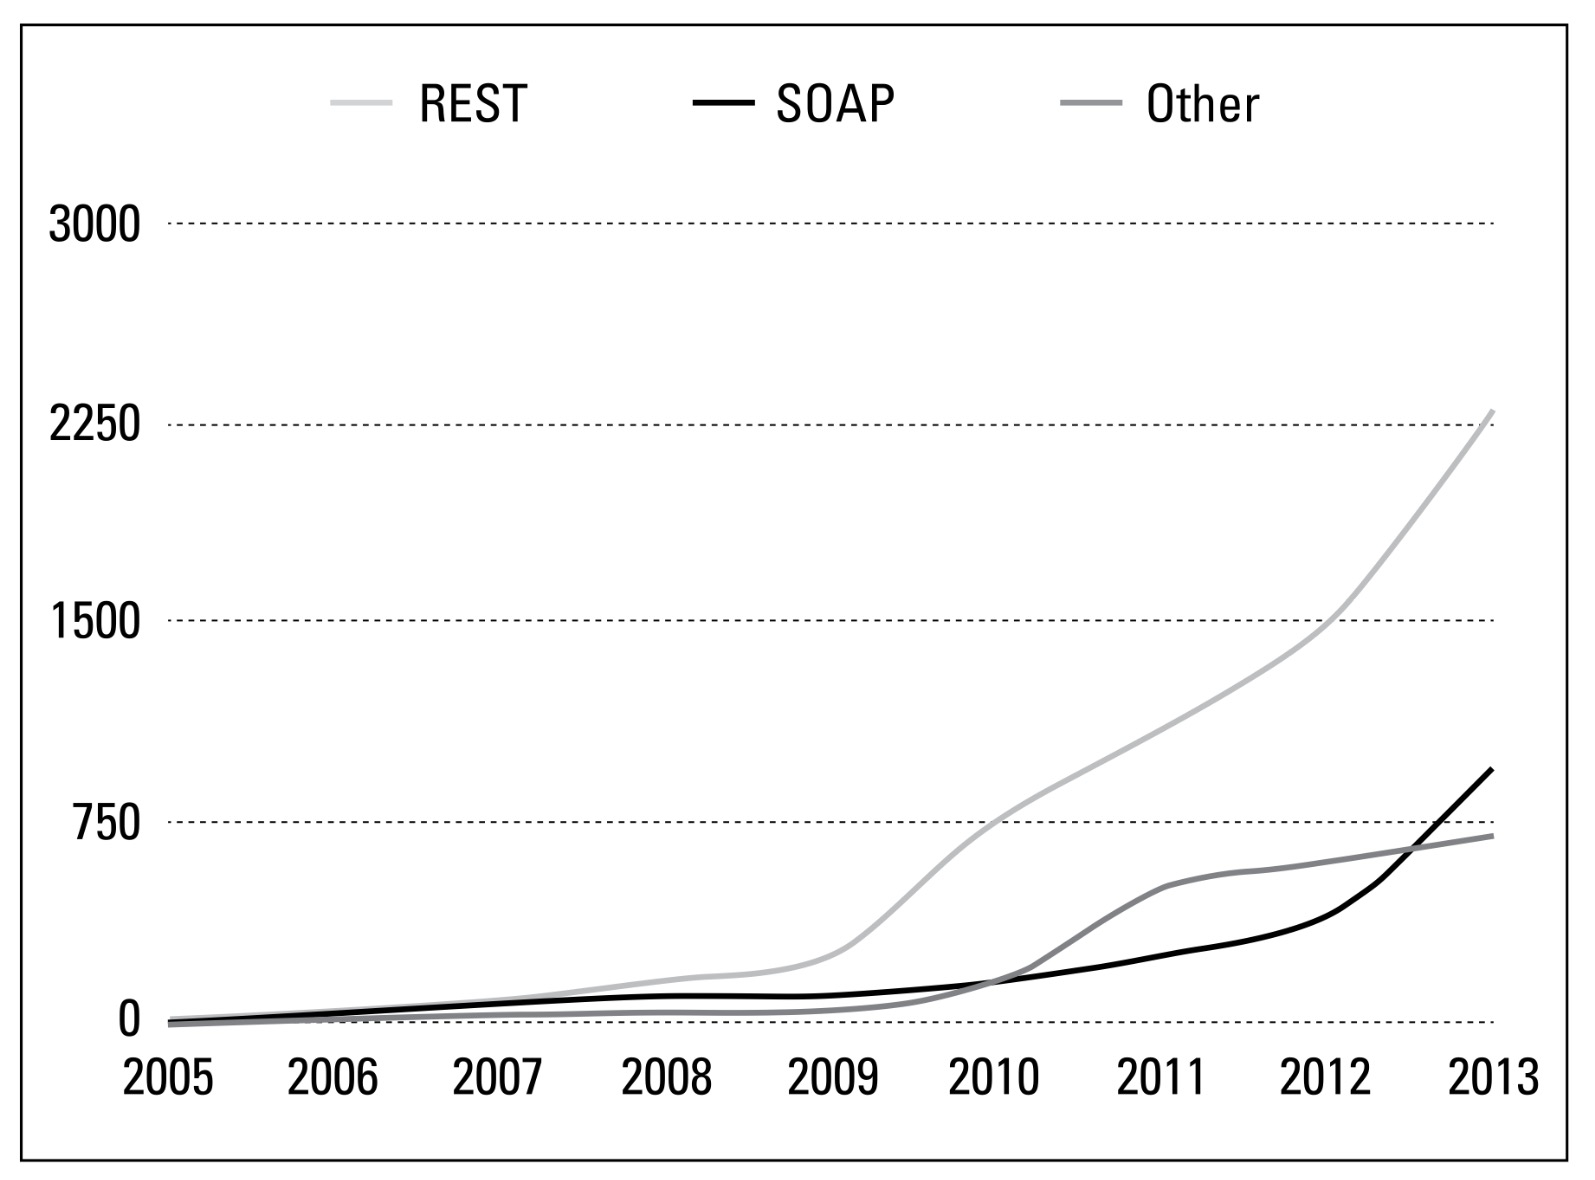
\includegraphics[width=\textwidth,height=\textheight,keepaspectratio]{figuras/api-styles.jpg}
  }
  \caption{Distribuição de estilos e protocolos para APIs}
\end{figure}

Sua maior vantagem de uso é por ser facilmente acessada por clientes web, mobile apps, dispositivos IoT. Isso permite que organizações construam clientes sem se preocupar com suporte à plataformas. Contudo, ao contrário de outros estilos de arquitetura, REST não sugere a criação de documentos de especificação, pois incentiva a escrita de respostas em hypertexo para navegação. Para Knupp, a idéia de documentação através de respostas autodescritivas dificulta a legibilidade, além de criar complexidade e informações adicionais. Ao invés, incentiva o uso de outras ferramentas de documentação e descrição de respostas. \cite{Knupp2016}

A seguir veremos sobre as restrições de arquitetura propostas pelo modelo REST, o que é uma API RESTful e seus níveis, além das atuais formas de documentação de APIs REST com suporte a leitura de máquinas.

\input{capitulos/fundamentos/rest/restricoes-de-arquitetura/index}
\input{capitulos/fundamentos/rest/restful/index}
\input{capitulos/fundamentos/rest/descricoes-de-api/index}

\section{GraphQL}

GraphQL é uma linguagem de consulta de dados e interpretador para APIs. Foi desenvolvida pela Facebook em 2012 mas sua especificação apenas publicada em 2015. Tem com objetivo fornecer uma descrição completa e compreensível dos dados disponíveis em APIs. Além disso, dá aos clientes o poder de trabalhar apenas com as estrutura de dados que precisam, torna mais fácil evoluir APIs ao longo do tempo e permite o desenvolvimento de ferramentas em cima de sua linguagem. \cite{GraphQL2016}

Importante ressaltar que GraphQL não está preso a algum banco de dados especifico ou mecanismo de armazenamento. Ao invés, é utilizado para consultar código já existente ou estruturas de dados. Para criar um esquema, é preciso definir os tipos de estruturas, seus campos de acesso e funções para mapear e retornar dados reais em código. \cite{GraphQL2016}

Por ser uma especificação, GraphQL possui implementações em diversas linguagens de programação e atualmente é usado em diversos contextos, sendo eles para comunicação entre cliente-servidor, microserviços, simplificação de APIs, navegação de árvores, gerador de consultas para banco de dados, entre outros.

\begin{figure}[h]
  \centering
  \inputminted[frame=single,framesep=10pt]{javascript}{anexos/graphql-schema.gql}
  \caption{Esquema GraphQL}
\end{figure}

\begin{figure}[h]
  \centering
  \inputminted[frame=single,framesep=10pt]{javascript}{anexos/graphql-code.js}
  \caption{API de um código em JavaScript}
\end{figure}

Uma vez que um serviço GraphQL está sendo executado (normalmente a uma URL em um serviço web), pode ser enviado consultas GraphQL para validar e executar. Uma consulta recebida é primeiro verificado para garantir que ele só se refere aos tipos e campos definidos, em seguida, executa as funções fornecidas para produzir um resultado. \cite{GraphQL2016}

\begin{figure}[h]
  \centering
  \inputminted[frame=single,framesep=10pt]{javascript}{anexos/graphql-query.gql}
  \caption{Query GraphQL para esquema}
\end{figure}

\begin{figure}[h]
  \centering
  \inputminted[frame=single,framesep=10pt]{javascript}{anexos/graphql-query-response.json}
  \caption{Resposta JSON da Query GraphQL}
\end{figure}

\input{capitulos/fundamentos/graphql/linguagem-de-consulta/index}
\input{capitulos/fundamentos/graphql/sistema-de-tipagem/index}
\input{capitulos/fundamentos/graphql/introspeccao/index}


\chapter{GraphQL}

GraphQL é, além de um interpretador, uma linguagem de consulta de dados criado pelo Facebook para trabalhar com API's de forma alternativa. Seu objetivo é fornecer uma descrição completa e compreensível de dados disponíveis em interfaces de aplicação. Assim, permitindo que clientes façam consultas de forma precisa em busca de dados que desejam trabalhar. \cite{GraphQL2016}

Por ser uma especificação recente, após sua publicação em 2015, GraphQL já apresenta implementações em diversas linguagens de programação e atualmente é utilizado em diversos contextos como na comunicação entre cliente-servidor, microserviços, navegação de árvores, gerador de consultas para banco de dados, entre outros.

É importante ressaltar que GraphQL não é uma linguagem de banco de dados, por mais que possa ser utilizado para esta finalidade. Ao invés, sua linguagem e interpretador trabalham com a ideia de mapeamento de campos e tipos de dados em aplicações, fornecendo uma interface unificada e amigável para desenvolvimento de produtos e de outras ferramentas, como a proposta neste trabalho. \cite{GraphQL2016}

Para gerar um esquema, antes é preciso que haja uma aplicação para que possa ser definido os tipos de estruturas, campos de acesso e funções de retorno de dados.

\begin{figure}[H]
  \centering
  \begin{minted}[frame=single,framesep=10pt,fontsize=\small]{javascript}
    var pessoa = {
      nome: "Mateus Maso"
    }

    class Query {
      pessoa() {
        return pessoa
      }
    }

    class Pessoa {
      nome(pessoa) {
        return pessoa.nome
      }
    }
  \end{minted}
  \caption{Exemplo de API em JavaScript (ES6)}
\end{figure}

\begin{figure}[H]
  \centering
  \begin{minted}[frame=single,framesep=10pt,fontsize=\small]{javascript}
    type Query {
      pessoa: User
    }

    type Pessoa {
      id: ID
      nome: String
    }
  \end{minted}
  \caption{Esquema GraphQL para API da Figura 11}
\end{figure}

Após a criação do esquema, já é possível enviar consultas GraphQL para que a ferramenta valide a semântica e sintaxe, transforme em execuções de API e retorne dados representados no formato JSON.  \cite{GraphQL2016}

\begin{figure}[H]
  \centering
  \begin{minted}[frame=single,framesep=10pt,fontsize=\small]{javascript}
    query {
      pessoa {
        nome
      }
    }
  \end{minted}
  \caption{Exemplo de consulta GraphQL para Figura 12}
\end{figure}

\begin{figure}[H]
  \centering
  \begin{minted}[frame=single,framesep=10pt,fontsize=\small]{javascript}
    {
      "pessoa": {
        "nome": "Mateus Maso"
      }
    }
  \end{minted}
  \caption{Resposta JSON esperada após execução pela Figura 13}
\end{figure}

A seguir, será feita uma abordagem sobre os elementos que compõem a linguagem, seu sistema de tipagem e como a analisar metadados de esquemas utilizando o processo de introspecção.

\section[Linguagem de Consulta]{Linguagem de Consulta}

Clientes que buscam realizar consultas de dados em esquemas GraphQL, antes precisam entender seu documento de requisição. Um documento GraphQL contém operações de consultas ou mutações, além de unidades de composição e reuso de consultas, descritas pelo nome de fragmentos. \cite{GraphQL2016} \\

\textbf{Sintaxe} \\

Documentos GraphQL são inspirados no formato de estrutura de dados JSON, porém sem seus valores e com alterações na sintaxe. Para que um esquema entenda um documento GraphQL, este deve descrever ao menos uma operação de consulta ou mutação. Uma operação de consulta é um processo de leitura da API. Já uma operação de mutação é representado por dois processos, uma escrita seguido de uma leitura na API.

Ao executar uma operação, deve-se expressar um conjunto de seleção de dados que se deseja receber. Este conjunto é representado por campos e fragmentos, onde um campo pode receber argumentos e deve descrever um dado ou subconjunto de dados. Isso permite explorar relacionamentos complexos através do profundo aninhamento de conjuntos de seleções em busca de retornar uma estrutura JSON parecida com o que se escreve na linguagem.

\begin{figure}[H]
  \centering
  \begin{minted}[frame=single,fontsize=\small]{javascript}
    query {
      pessoa(id: 4) {
        id
        nome
        sobrenome
        nascimento: aniversario {
          mes
          dia
        }
        amigos(limite: 10) {
          nome
        }
      }
    }
  \end{minted}
  \caption{Exemplo de seleção em consultas GraphQL}
\end{figure}

\textbf{Fragmentos} \\

Fragmentos são a principal unidade de composição em GraphQL, pois permitem o reuso de seleção de campos que se repetem em documentos. É representado por um nome, seguido pelo tipo que está sendo aplicado a seleção de campos. Podem também ser expressos de forma "inline", onde não a a necessidade de definir um nome.

\begin{figure}[H]
  \centering
  \begin{minted}[frame=single,framesep=10pt,fontsize=\small]{javascript}
    query {
      pessoa(id: 4) {
        id
        ...identidade
        ...relacionamentos
      }
    }

    fragment identidade on Pessoa {
      nome
      sobrenome
      nascimento: aniversario {
        mes
        dia
      }
    }

    fragment relacionamentos on Pessoa {
      amigos(limite: 10) {
        nome
      }
    }
  \end{minted}
  \caption{Exemplo da figura 14 utilizando fragmentos}
\end{figure}

\section[Sistema de Tipagem]{Sistema de Tipagem}

Para descrever um esquema GraphQL a partir de uma API, antes é preciso fazer o uso de seu sistema de tipagem. Através da abstração de entidades de um serviço, representa-se um conjunto finito de tipos para ser acessado por documentos GraphQL. Um tipo é uma forma de representação de dados especifico da linguagem de definição para que a ferramenta saiba como interpretar operações de consulta e mutação.

Durante o processo de mapeamento de entidades, faz-se a conversão de estruturas de dados em conjuntos dos tipos folha, de acondicionamento, de composição e abstratos. Um tipo folha é representado por valores finais, singulares e não nulos da estrutura, onde os tipos de acondicionamento e composição são utilizados em cima dos tipos folha para alterar o comportamento e combinar outros tipos em busca da representação de estruturas mais complexas. Por fim, existem os tipos abstratos, que servem para reusar os tipos anteriores através do uso de conceitos alto nível.

\begin{table}[H]
  \centering
  \begin{tabular}{|c|c|c|c|c|}
    \hline
    Tipo & Classificação \\
    \hline
    Enum & Folha \\
    \hline
    Int & Folha \\
    \hline
    Float & Folha \\
    \hline
    String & Folha \\
    \hline
    Boolean & Folha \\
    \hline
    ID & Folha \\
    \hline
    Object & Composição \\
    \hline
    Union & Abstrato \\
    \hline
    Interface & Abstrato \\
    \hline
    Non-Null & Acondicionamento \\
    \hline
  	List & Acondicionamento \\
    \hline
  \end{tabular}
  \caption{Classificação de tipos GraphQL}
\end{table}

Após a conversão de estruturas de dados em tipos GraphQL, para que estes também sejam acessados por documentos, é preciso incluí-los em um tipo de composição especial definido pelo esquema chamado "root". Dessa forma, é possível modelar os primeiros campos de acesso que o esquema deseja disponibilizar para que clientes façam a execução de operações a partir deles.

\begin{figure}[H]
  \centering
  \begin{minted}[frame=single,framesep=10pt,fontsize=\small]{javascript}
    interface Individuo {
      nome: String
    }

    type Pessoa implements Individuo {
      foto: Foto
      amigos: [Pessoa]
    }

    type Foto {
      url: String
    }

    union Resultado = Foto | Pessoa

    type Pesquisa {
      resultado: Resultado
    }
  \end{minted}
  \caption{Exemplo de representação do esquema da Figura 17}
\end{figure}

\begin{figure}[H]
  \centering
  \begin{minted}[frame=single,framesep=10pt,fontsize=\small]{javascript}
    var IndividuoType = new GraphQLInterfaceType({
      fields: {
        nome: {type: GraphQLStringType}
      }
    })

    var PessoaType = new GraphQLObjectType({
      interfaces: [IndividuoType],
      fields: () => {
        return {
          foto: {type: FotoType},
          amigos: {type: [PessoaType]}
        }
      }
    })

    var FotoType = new GraphQLObjectType({
      fields: {
        url: {type: GraphQLStringType}
      }
    })

    var ResultadoType = new GraphQLUnionType({
      types: [PessoaType, FotoType]
    })

    var PesquisaType = new GraphQLObjectType({
      fields: {
        resultado: {type: ResultadoType}
      }
    })

    var schema = new GraphQLSchema({
      query: new GraphQLObjectType({
        fields: {
          pesquisa: {type: PesquisaType}
        }
      })
    })
  \end{minted}
  \caption{Implementação JavaScript da Figura 17}
\end{figure}

\section[Introspecção]{Introspecção}

Em GraphQL, o termo introspecção refere-se à uma consulta especial usada na busca por metadados de esquemas. Uma das vantagens desta funcionalidade está na possibilidade de ferramentas usá-la para gerar código, documentação, prever mudanças, alertar de campos deprecados, entre outras aplicações. Isso torna GraphQL uma ótima opção como estilo de arquiteturas em sistemas distribuídos, pois apresenta de forma "nativa" uma poderosa linguagem de descrição de serviços.

\begin{figure}[H]
  \centering
  \begin{minted}[frame=single,framesep=10pt,fontsize=\footnotesize]{javascript}
    query introspeccao {
      __schema {
        queryType { name }
        mutationType { name }
        types {
          kind
          name
          description
          fields {
            name
            description
          }
        }
      }
    }
  \end{minted}
  \caption{Introspecção}
\end{figure}


\chapter{Desenvolvimento}

Contextualizar o projeto desenvolvido com os fundamentos apresentados. Dizer que nos prox subcapítulos são descritos o processo de planejamento de projeto, detalhes de implementação e a etapa de validação sobre o impacto da ferramenta no processo de mudança no fluxo de dados pelo servidor.

\tikzstyle{decision} = [diamond, draw, fill=blue!20, 
    text width=4.5em, text badly centered, node distance=3cm, inner sep=0pt]
\tikzstyle{block} = [rectangle, draw, fill=blue!20, 
    text width=5em, text centered, rounded corners, minimum height=4em]
\tikzstyle{line} = [draw, -latex']
\tikzstyle{cloud} = [draw, ellipse,fill=red!20, node distance=3cm,
    minimum height=2em]

\section{Planejamento de Projeto}

Explicar o processo de idealização, definição de interface e fluxo de execução da ferramenta (control flow).  \\ 

\textbf{Processo de idealização} \\

\begin{enumerate}
\item Por que é difícil realizar mudanças de fluxo de dados no servidor para ganho de performance? Porque clientes estão acoplados em um contrato de acesso à interface de aplicação.
\item Como evitar quebrar clientes devido à mudança no fluxo de dados? Evitar que clientes façam contrato de acesso direto à API através de requisições explícitas.
\item Como evitar que clientes façam acesso direto à API? Usando uma ferramenta que seja responsável por intermediar esse acesso de dados em APIs.
\item De que forma ocorre essa intermediação? Usando uma linguagem para expressar as estruturas de dados que o cliente precisa.
\item Existe uma linguagem completa para isso? Sim, ela se chama GraphQL.
\item É possível utilizar GraphQL em um ambiente de cliente? Sim, ela foi desenvolvida para ser "isomorphic", além disso, não requer a implementação de interpretadores no servidor.
\item Como tu vai analisar e mapear essas consultas de linguagem em requisições para o servidor? Através de um sistema chamado AST.
\item O que é AST? São árvores sintáticas abstratas, usadas para trabalhar com a consulta da linguagem em forma de estrutura de dados.
\item O que me garante que esse AST será convertido em requisições performáticas? Através da analise de estruturas de dados disponíveis no servidor e como acessar.
\item Como vai ser o algoritmo de escolha de rota? Através da redução de ASTs, ou seja, analisando as estruturas de dados disponíveis e seu acesso e transformando o AST através de uma heurística que usa como variáveis o número de dados usados e dados não usados de retorno em uma requisição.
\item Como tu vai saber quais estruturas de dados estão disponíveis no servidor (API) e de que forma são acessados? Através de formatos de descrição de API. APIs que possuem a habilidade de representar metadados podem ser usadas pela ferramenta.
\end{enumerate}

\textbf{Definição de interface} \\

Falar sobre o nome da ferramenta. Dizer que o propósito da ferramenta é ser um gerador de esquema GraphQL através de configurações de serviços (API's), que seja possível ser executado pela função GraphQL e é responsável por interpretar a consulta em requisições para API's. Além disso que seja adaptável pra outros tipo de descrição serviços. Falar sobre o adaptador HyperSchema para usar em APIs REST e RESTful.

\begin{enumerate}
\item Definir serviços
\item Gerar esquema a partir dos serviços
\item Executar consultas usando o esquema gerado
\end{enumerate}

\begin{figure}[H]
  \centering
  \begin{minted}[frame=single,framesep=10pt,fontsize=\small]{javascript}
    import {adapter} from "graphql-jay-hyperschema"
  
    export function v1() {
      return fetch("/api/v1/schema").then((response) => {
        return response.json()
      }).then((schema) => {
        return {
          url: "/api/v1",
          schema,
          adapter,
          wrapper: {}
        }
      })
    }
  \end{minted}
  \caption{Serviço REST com adaptador de JSON Hyper-Schema}
\end{figure}

\begin{figure}[H]
  \centering
  \begin{minted}[frame=single,framesep=10pt,fontsize=\small]{javascript}
    import {graphql} from "graphql"
    import {composeSchema} from "graphql-jay"
    import services from "./services"
    
    composeSchema(...services).then((schema) => {
      graphql(schema, "{ user { id } }").then((response) => { 
        console.log(response.data)
      })
    })
  \end{minted}
  \caption{Exemplo de criação de esquema e execução}
\end{figure}

\textbf{Fluxo de execução} \\

Existem dois fluxos, o primeiro é de criação de esquema. O segundo é de execução do esquema.

\begin{figure}[H]
  \centering
  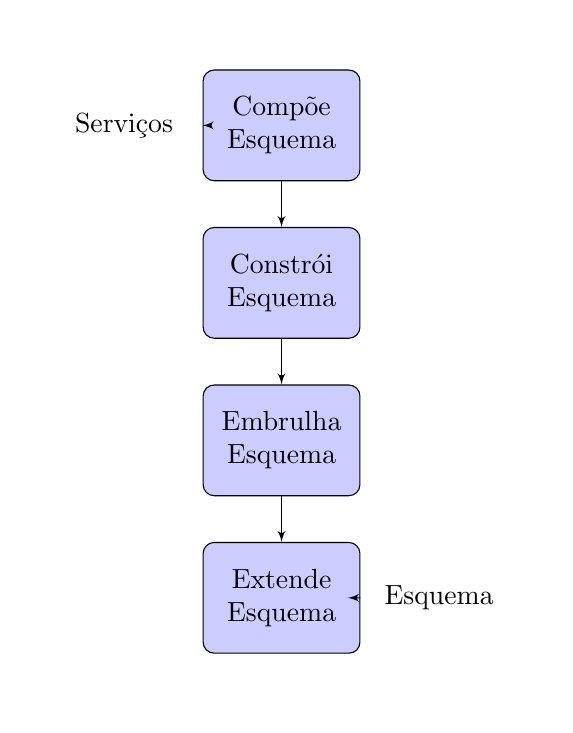
\begin{tikzpicture}[node distance = 2cm, auto]
    \node [block] (composeSchema) {Compõe Esquema};
    \node [cloud, left of=composeSchema] (services) {Serviços};
    \node [block, below of=composeSchema] (buildSchema) {Constrói Esquema};
    \node [block, below of=buildSchema] (wrapSchema) {Embrulha Esquema};
    \node [block, below of=wrapSchema] (deepExtendSchema) {Extende Esquema};
    \node [cloud, right of=deepExtendSchema] (schema) {Esquema};
    \path [line] (composeSchema) -- (buildSchema);
    \path [line] (buildSchema) -- (wrapSchema);
    \path [line] (wrapSchema) -- (deepExtendSchema);
    \path [line,dashed] (services) -- (composeSchema);
    \path [line,dashed] (deepExtendSchema) -- (schema);
  \end{tikzpicture}
  \caption{Criação de esquema}
\end{figure}

\begin{figure}[H]
  \centering
  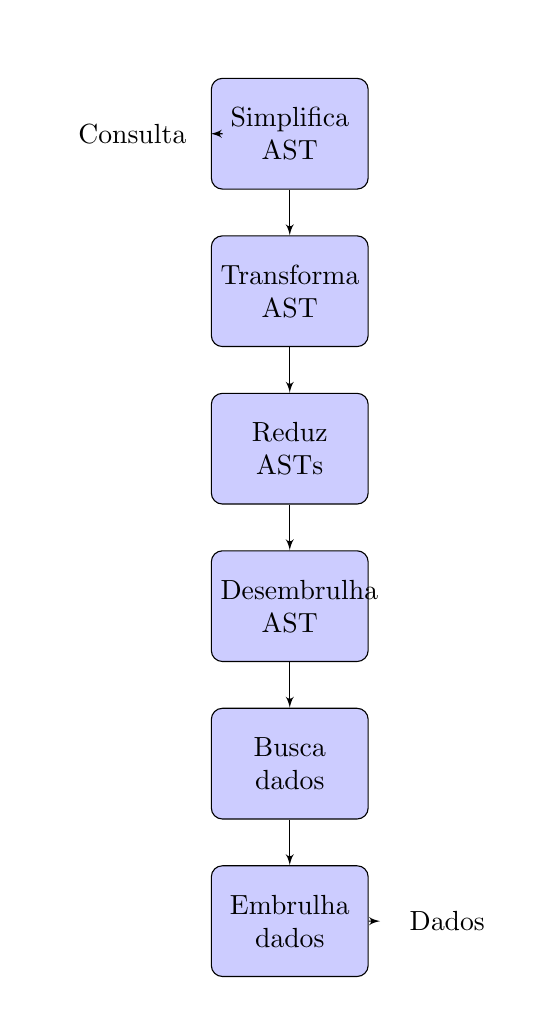
\begin{tikzpicture}[node distance = 2cm, auto]
    \node [block] (simplifyAST) {Simplifica AST};
    \node [cloud, left of=simplifyAST] (services) {Consulta};
    \node [block, below of=simplifyAST] (transformAST) {Transforma AST};
    \node [block, below of=transformAST] (reduceASTs) {Reduz ASTs};
    \node [block, below of=reduceASTs] (unwrapAST) {Desembrulha AST};
    \node [block, below of=unwrapAST] (fetchData) {Busca dados};
    \node [block, below of=fetchData] (wrapData) {Embrulha dados};
    \node [cloud, right of=wrapData] (schema) {Dados};
    \path [line] (simplifyAST) -- (transformAST);
    \path [line] (transformAST) -- (reduceASTs);
    \path [line] (reduceASTs) -- (unwrapAST);
    \path [line] (unwrapAST) -- (fetchData);
    \path [line] (fetchData) -- (wrapData);
    \path [line,dashed] (services) -- (simplifyAST);
    \path [line,dashed] (wrapData) -- (schema);
  \end{tikzpicture}
  \caption{Execução de consulta}
\end{figure}


\section{Implementação}

A partir da definição de interface e fluxo de execução, foram implementados dez funções no total. Quatro delas responsáveis por gerar o esquema. Três para analisar o AST da consulta e outras três para transformar o AST em requisições para API de cada serviço. Além disso, três dessas funções são extensíveis através de adaptadores para análise diferentes formatos para descrição de metadados em APIs. 

A seguir, é descrito brevemente as 3 categorias de funções, junto com seu objetivo e a assinatura de cada método escrito em JavaScript. \\

\textbf{Funções para composição de esquema} \\

Representam quatro funções e seu principal objetivo é compor, de forma assíncrona, um esquema GraphQL unificado a partir dos metadados de cada serviço.

\begin{figure}[H]
  \centering
  \begin{minted}[frame=single,framesep=10pt,fontsize=\footnotesize]{text}
  function composeSchema(
    services: [Service]
  ): Promise<GraphQLSchema>

  function buildSchema(
    schema: JSON
  ): Promise<GraphQLSchema>

  function wrapSchema(
    schema: GraphQLSchema, 
    wrapper: Wrapper
  ): Promise<GraphQLSchema>

  function deepExtendSchema(
    schemas: [GraphQLSchema]
  ): Promise<GraphQLSchema>
  \end{minted}
  \caption{Assinatura das funções para composição de esquema}
\end{figure}

\textbf{Funções para análise de AST} \\

São três funções que buscam analisar o AST gerado pela consulta GraphQL através de um algoritmo que transforma e reduz este em um AST específico e performático para cada serviço.

\begin{figure}[H]
  \centering
  \begin{minted}[frame=single,framesep=10pt,fontsize=\footnotesize]{text}
  function simplifyAST(
    value: AST, 
    info: JSON
  ): SimplifiedAST

  function transformAST(
    schema: JSON,
    clientSchema: GraphQLSchema, 
    ast: SimplifiedAST
  ): SimplifiedAST

  function reduceASTs(
    rootAST: SimplifiedAST, 
    asts: [SimplifiedAST]
  ): void
  \end{minted}
  \caption{Assinatura das funções para análise de AST}
\end{figure}

\textbf{Funções para busca de dados} \\

São as três últimas funções responsáveis por converter os ASTs produzidos na categoria de análise em requisições para API de cada serviço.

\begin{figure}[H]
  \centering
  \begin{minted}[frame=single,framesep=10pt,fontsize=\footnotesize]{text}
  function unwrapAST(
    ast: SimplifiedAST, 
    schema: GraphQLSchema, 
    wrapper: Wrapper
  ): SimplifiedAST

  function fetchData(
    schema: JSON, 
    ast: SimplifiedAST, 
    url: string
  ): Promise<JSON>

  function wrapData(
    data: JSON, 
    schema: JSON, 
    wrapper: Wrapper
  ): Promise<JSON>
  \end{minted}
  \caption{Assinatura das funções para busca de dados}
\end{figure}

\section{Validação}



\begin{enumerate}
\item Teste 1
\item Teste 2
\item Teste 3
\item Teste 4
\item Teste 5
\item Teste 6
\end{enumerate}

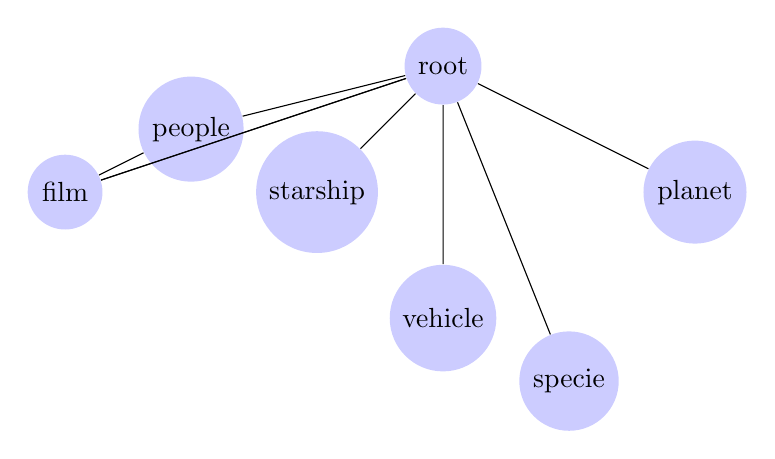
\begin{tikzpicture}
  [scale=.8,auto=left,every node/.style={circle,fill=blue!20}]
  \node (n1) at (6,10) {root};
  \node (n2) at (0,8)  {film};
  \node (n3) at (2,9)  {people};
  \node (n4) at (4,8) {starship};
  \node (n5) at (6,6)  {vehicle};
  \node (n6) at (8,5)  {specie};
  \node (n7) at (10,8)  {planet};

  \foreach \from/\to in {n1/n2,n1/n2,n1/n3,n1/n4,n1/n5,n1/n6,n1/n7,n2/n3}
    \draw (\from) -- (\to);

\end{tikzpicture}


\chapter{Resultados}

% \begin{tikzpicture}
% [
%     pie chart,
%     slice type={comet}{blu},
%     slice type={legno}{rosso},
%     slice type={coltello}{giallo},
%     slice type={sedia}{viola},
%     slice type={caffe}{verde},
%     pie values/.style={font={\small}},
%     scale=2
% ]

%     \pie{2008}{73/comet,13/legno,7/sedia,7/coltello}
%     \pie[xshift=2.2cm,values of coltello/.style={pos=1.1}]%
%         {2009}{52/comet,23/legno,17/sedia,3/coltello,5/caffe}
%     \pie[xshift=4.4cm,values of caffe/.style={pos=1.1}]%
%         {2010}{56/comet,26/legno,9/sedia,7/coltello,2/caffe}

%     \legend[shift={(0cm,-1cm)}]{{Comet (Pordenone)}/comet, {Wood and furniture (Livenza)}/legno, {Knife (Maniago)}/coltello}
%     \legend[shift={(3cm,-1cm)}]{{Chair (Manzano)}/sedia, {Coffee (Trieste)}/caffe}
% \end{tikzpicture}

\begin{figure}[H]
  \centering
  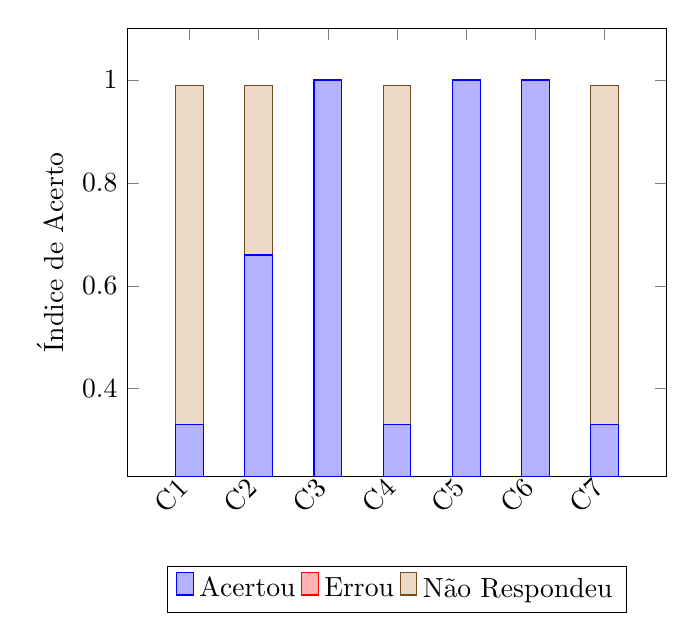
\begin{tikzpicture}
  \begin{axis}[
      ybar stacked,
      enlargelimits=0.15,
      legend style={at={(0.5,-0.20)},
        anchor=north,legend columns=-1},
      ylabel={Índice de Acerto},
      symbolic x coords={C1, C2, C3, C4, 
          C5, C6, C7},
      xtick=data,
      x tick label style={rotate=45,anchor=east},
      ]
  \addplot+[ybar] plot coordinates {(C1,0.33) (C2,0.66) 
    (C3,1) (C4,0.33) (C5,1) (C6,1) (C7,0.33)};
  \addplot+[ybar] plot coordinates {(C1,0) (C2,0) 
    (C3,0) (C4,0) (C5,0) (C6,0) (C7,0)};
  \addplot+[ybar] plot coordinates {(C1,0.66) (C2,0.33) 
    (C3,0) (C4,0.66) (C5,0) (C6,0) (C7,0.66)};
  \legend{Acertou, Errou, Não Respondeu}
  \end{axis}
  \end{tikzpicture}
  \caption{Índice de acerto sem o uso da ferramenta}
\end{figure}

\begin{figure}[H]
  \centering
  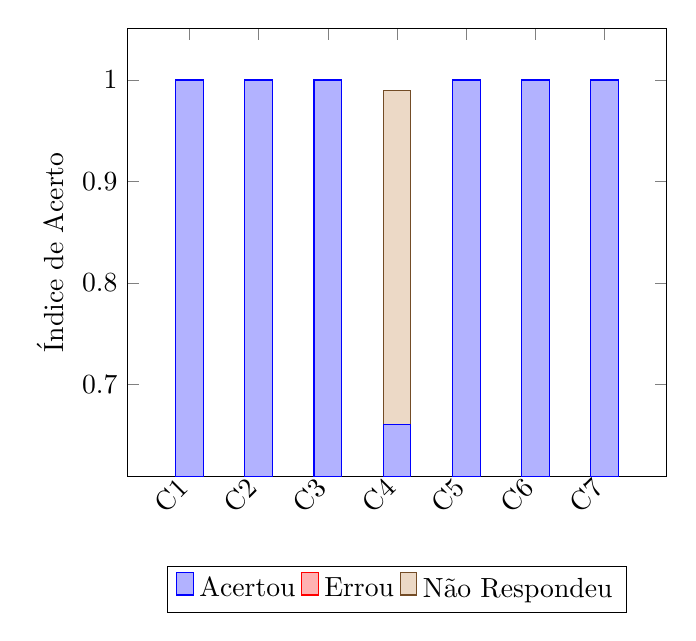
\begin{tikzpicture}
  \begin{axis}[
      ybar stacked,
      enlargelimits=0.15,
      legend style={at={(0.5,-0.20)},
        anchor=north,legend columns=-1},
      ylabel={Índice de Acerto},
      symbolic x coords={C1, C2, C3, C4, 
          C5, C6, C7},
      xtick=data,
      x tick label style={rotate=45,anchor=east},
      ]
  \addplot+[ybar] plot coordinates {(C1,1) (C2,1) 
    (C3,1) (C4,0.66) (C5,1) (C6,1) (C7,1)};
  \addplot+[ybar] plot coordinates {(C1,0) (C2,0) 
    (C3,0) (C4,0) (C5,0) (C6,0) (C7,0)};
  \addplot+[ybar] plot coordinates {(C1,0) (C2,0) 
    (C3,0) (C4,0.33) (C5,0) (C6,0) (C7,0)};
  \legend{Acertou, Errou, Não Respondeu}
  \end{axis}
  \end{tikzpicture}
  \caption{Índice de acerto com o uso da ferramenta}
\end{figure}

% \begin{tikzpicture}
% \pgfplotsset{every axis legend/.append style={
% 		at={(0.5,1.03)},
% 		anchor=south}}
% \begin{axis}[legend columns=4]
% \addplot coordinates {(1,0.33) (2,0.66) (3,1) (4,0.33) (5,1) (6,1) (7,0.33)};
% \addplot coordinates {(1,1) (2,1) (3,1) (4,1) (5,1) (6,1) (7,1)};
% \legend{Cliente 1,Cliente 2}
% \end{axis}
% \end{tikzpicture}

\begin{figure}[H]
  \centering
  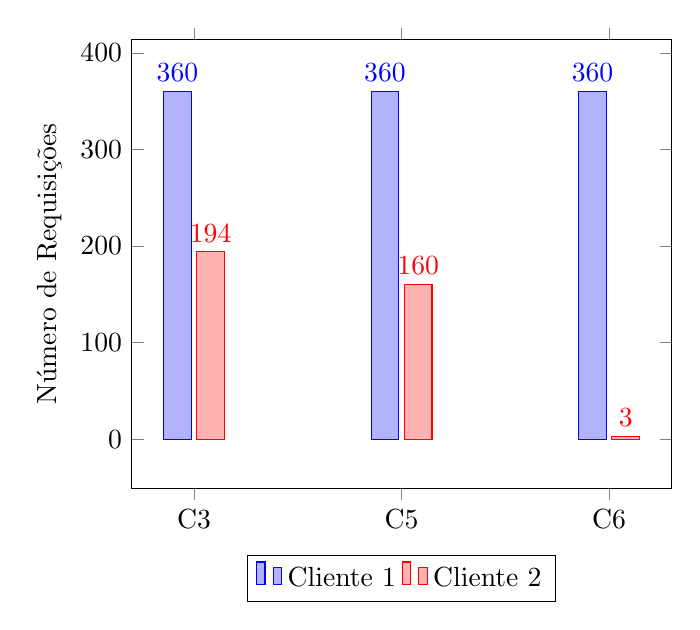
\begin{tikzpicture}
  \begin{axis}[
      ybar,
      enlargelimits=0.15,
      legend style={at={(0.5,-0.15)},
        anchor=north,legend columns=-1},
      ylabel={Número de Requisições},
      symbolic x coords={C3,C5,C6},
      xtick=data,
      nodes near coords,
      nodes near coords align={vertical},
      ]
  \addplot coordinates {(C3,360) (C5,360) (C6,360)};
  \addplot coordinates {(C3,194) (C5,160) (C6,3)};
  \legend{Cliente 1,Cliente 2}
  \end{axis}
  \end{tikzpicture}
  \caption{Comparação no número de requisições das mudanças OK}
\end{figure}

\begin{figure}[H]
  \centering
  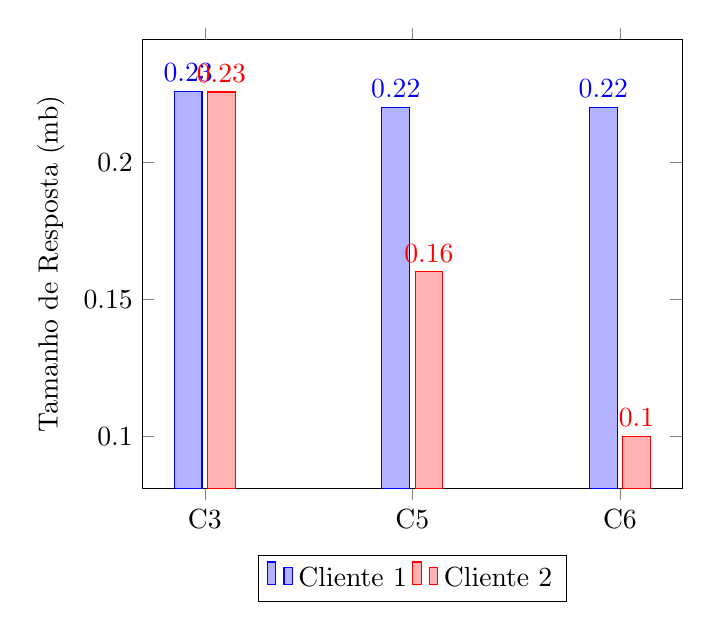
\begin{tikzpicture}
  \begin{axis}[
      ybar,
      enlargelimits=0.15,
      legend style={at={(0.5,-0.15)},
        anchor=north,legend columns=-1},
      ylabel={Tamanho de Resposta (mb)},
      symbolic x coords={C3,C5,C6},
      xtick=data,
      nodes near coords,
      nodes near coords align={vertical},
      ]
  \addplot coordinates {(C3,0.225777) (C5,0.22) (C6,0.22)};
  \addplot coordinates {(C3,0.225572) (C5,0.16) (C6,0.10)};
  \legend{Cliente 1,Cliente 2}
  \end{axis}
  \end{tikzpicture}
  \caption{Comparação no tamanho de resposta das mudanças OK}
\end{figure}

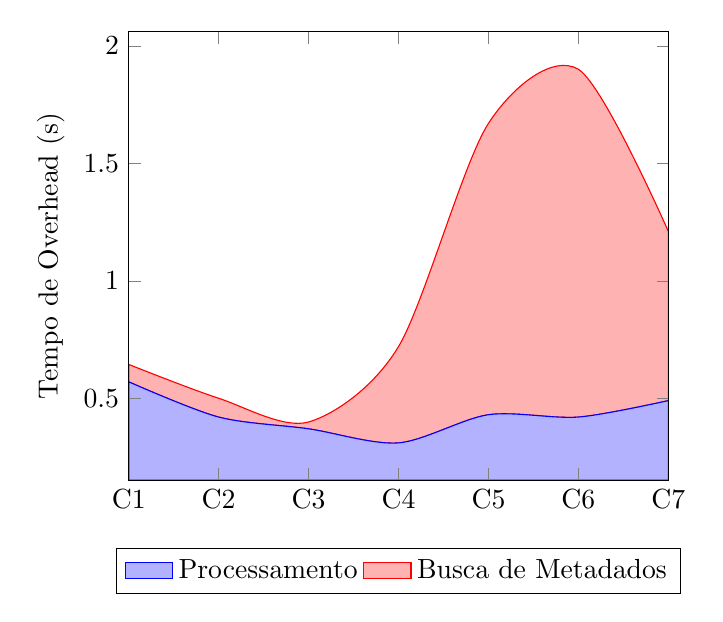
\begin{tikzpicture}
	\begin{axis}[
        ylabel={Tempo de Overhead (s)},
        legend style={at={(0.5,-0.15)},
        anchor=north,legend columns=-1},
		smooth,
		stack plots=y,
		area style,
        symbolic x coords={C1,C2,C3,C4,C5,C6,C7},
		enlarge x limits=false]
	\addplot coordinates
		{(C1,0.57) (C2,0.42) (C3,0.37) (C4,0.31) (C5,0.43) (C6,0.42) (C7,0.49)} 
		\closedcycle;
	\addplot coordinates
		{(C1,0.074) (C2,0.08) (C3,0.029) (C4,0.41) (C5,1.24) (C6,1.48) (C7,0.72)}
		\closedcycle;
    \legend{Processamento,Busca de Metadados}
	\end{axis}
\end{tikzpicture}

% Conclusão

\chapter{CONCLUSÃO}

As conclusões devem responder às questões da pesquisa,
em relação aos objetivos e hipóteses.
Devem ser breves
podendo apresentar recomendações
e sugestões para trabalhos futuros.


\bibliographystyle{abnt-alf}
\bibliography{bibliografia/index}
\anexo
\chapter{Código Fonte}

\end{document}
